% !TeX program = lualatex
% Separate revision: model/math -> PINNs and identifiability -> neural-mechanistic hybrid.
% The original regulatory schematic is included unchanged.
\documentclass[final]{beamer}
\usepackage[size=custom,width=121.92,height=91.44,scale=1.0]{beamerposter}
\usepackage{fontspec}
\usepackage{amsmath,amssymb,booktabs,array,graphicx}
\usepackage{tikz}
\usetikzlibrary{calc,arrows.meta}
\usefonttheme{professionalfonts}
\defaultfontfeatures{Ligatures=TeX}
\setsansfont{TeX Gyre Heros}
\setmainfont{TeX Gyre Pagella}
\newfontfamily\Display{TeX Gyre Pagella}
\definecolor{Ink}{HTML}{152A3A}
\definecolor{Muted}{HTML}{596570}
\definecolor{Garnet}{HTML}{78253B}
\definecolor{Paper}{HTML}{F5F3EF}
\definecolor{Rule}{HTML}{D4CDC7}
\definecolor{PaleBlue}{HTML}{ECF2F6}
\definecolor{DataBlue}{HTML}{1F77B4}
\definecolor{DataOrange}{HTML}{FF7F0E}
\definecolor{DataRed}{HTML}{CC3333}
\setbeamercolor{normal text}{fg=Ink,bg=Paper}
\setbeamertemplate{navigation symbols}{}
\setbeamertemplate{headline}{}
\setbeamertemplate{footline}{}
\hypersetup{pdftitle={Identifiability and Experimental Design for Neural-Mechanistic Hybrid Models Using Physics-Informed Neural Networks in Colorectal Cancer},
 pdfauthor={Amirkhan Aidarkhan; Pascal K. Kataboh},colorlinks=true,urlcolor=Ink}
\title{Identifiability and Experimental Design for Neural-Mechanistic Hybrid Models Using Physics-Informed Neural Networks in Colorectal Cancer}
\newlength{\Margin}\setlength{\Margin}{1.1in}
\newlength{\Gutter}\setlength{\Gutter}{.75in}
\newlength{\LeftWidth}\setlength{\LeftWidth}{15.1in}
\newlength{\MiddleWidth}\setlength{\MiddleWidth}{14.6in}
\newlength{\RightWidth}\setlength{\RightWidth}{14.6in}
\newlength{\LiveWidth}\setlength{\LiveWidth}{45.8in}
\newlength{\TitleTop}\setlength{\TitleTop}{1.0in}
\newlength{\LogoPanelWidth}\setlength{\LogoPanelWidth}{4.8in}
\newlength{\LogoPanelHeight}\setlength{\LogoPanelHeight}{2.95in}
\newlength{\LogoWidth}\setlength{\LogoWidth}{4.1in}
\newlength{\TitleGap}\setlength{\TitleGap}{.6in}
\newlength{\TitleWidth}\setlength{\TitleWidth}{\dimexpr\LiveWidth-\LogoPanelWidth-\TitleGap\relax}
\newcommand{\Aff}[1]{\textsuperscript{#1}}
\newlength{\BodyTop}\setlength{\BodyTop}{4.6in}
\newlength{\BodyHeight}\setlength{\BodyHeight}{29.45in}
\newlength{\FooterTop}\setlength{\FooterTop}{34.4in}
\newcommand{\BodyFont}{\fontsize{28}{36}\selectfont}
\newcommand{\CaptionFont}{\fontsize{24}{31}\selectfont}
\newcommand{\TableFont}{\fontsize{26}{34}\selectfont}
\newcommand{\SectionBar}[1]{%
  \noindent\begingroup\setlength{\fboxsep}{16pt}%
  \colorbox{Garnet}{\parbox{\dimexpr\linewidth-32pt\relax}{%
    \Display\bfseries\color{white}\fontsize{35}{43}\selectfont
    #1}}%
  \endgroup\par\vspace{16pt}}
\newcommand{\SectionTitle}[2]{\SectionBar{#1\enspace #2}}
\newcommand{\Subhead}[1]{\par\vspace{18pt}%
  {\Display\bfseries\color{Garnet}\fontsize{33}{40}\selectfont #1\par}%
  \vspace{6pt}{\color{Rule}\hrule height 1pt}\vspace{12pt}}
\newcommand{\Caption}[1]{\par\vspace{7pt}{\CaptionFont #1\par}}
\newsavebox{\MathBox}
\newcommand{\Equation}[2]{\par\vspace{9pt}\begingroup
  \fontsize{32}{42}\selectfont
  \sbox{\MathBox}{$\displaystyle #2$}%
  \ifdim\wd\MathBox>\dimexpr\linewidth-68pt\relax
    \PackageError{poster}{Equation #1 is too wide}{Break the equation into aligned lines.}
  \fi
  \noindent\makebox[\linewidth]{\usebox{\MathBox}}\llap{\CaptionFont(#1)}%
  \par\endgroup\vspace{8pt}}
\newcommand{\PanelStart}[1]{%
  \begin{minipage}[t]{#1}\BodyFont\raggedright
  \setlength{\parindent}{0pt}\setlength{\parskip}{5pt}%
  \setlength{\abovedisplayskip}{8pt}\setlength{\belowdisplayskip}{8pt}%
  \setlength{\abovedisplayshortskip}{0pt}\setlength{\belowdisplayshortskip}{6pt}}
\newcommand{\PanelEnd}{\end{minipage}}
\newsavebox{\TitleBox}\newsavebox{\LeftColumn}
\newsavebox{\MiddleColumn}\newsavebox{\RightColumn}\newsavebox{\FooterBox}
\newcommand{\CheckHeight}[3]{%
  \typeout{POSTER-HEIGHT #1: \the\dimexpr\ht#2+\dp#2\relax; limit #3}%
  \ifdim\dimexpr\ht#2+\dp#2\relax>#3\relax
    \PackageError{poster}{#1 exceeds its allotted height}{Shorten content or adjust layout.}
  \fi}
\begin{document}
% Generated from saved results by figures/make_figures.py.

\newcommand{\FisherCompactRows}{%
Normal & 13 & 22 & 1 \\
Early & 17 & 18 & 1 \\
Advanced & 14 & 20 & 2 \\
Severe & 14 & 21 & 1 \\
}

\newcommand{\UntreatedMYCError}{%
0.31
}

\newcommand{\UntreatedAPCError}{%
0.75
}

\newcommand{\TreatedMYCError}{%
0.40
}

\newcommand{\TreatedAPCError}{%
0.54
}

\newcommand{\ForwardRows}{%
Dense supervised & 100 & 1.06\% \\
Sparse PINN & 40 & 2.41\% \\
}

\newcommand{\ForwardDenseError}{%
1.06
}

\newcommand{\ForwardSparseError}{%
2.41
}

\newcommand{\InverseRows}{%
Normal & 16 & 17 & +1 \\
Early Adenoma & 9 & 16 & +7 \\
Advanced Adenoma & 6 & 10 & +4 \\
Severe APC Loss & 6 & 7 & +1 \\
}

\newcommand{\InverseCompactRows}{%
Autodiff & 16 & 9 & 6 & 6 & 37 \\
Integral & 17 & 16 & 10 & 7 & 50 \\
}

\newcommand{\AutodiffTotal}{%
37
}

\newcommand{\IntegralTotal}{%
50
}

\newcommand{\HybridRows}{%
RA $\to$ HOXA5 & 51/136 & 53/136 & 7.6–23.7 \\
$\beta$-catenin $\to$ MYC & 48/136 & 43/136 & 6.2–9.5 \\
APC loss & 52/140 & 53/140 & 0.12 \\
}

\newcommand{\DoseRows}{%
$a_M$ & WNT depletion & 2.17 & 1.55 \\
$a_M$ & WNT + HOXA13 suppression & 0.02 & 0.01 \\
}

\newcommand{\ProtocolRows}{%
$a_{13}$ & none & 12.84 & 95.56 \\
$a_{13}$ & $\beta$-catenin depletion & 51.52 & 59.84 \\
$a_{13}$ & MYC depletion & 0.11 & 0.05 \\
}

\sbox{\TitleBox}{\begin{minipage}{\TitleWidth}\raggedright\color{white}
  \setlength{\parindent}{0pt}
  {\Display\bfseries\fontsize{62}{70}\selectfont
  Identifiability and Experimental Design for Neural-Mechanistic Hybrid Models\\
  Using Physics-Informed Neural Networks in Colorectal Cancer\par}
  \vspace{10pt}
  {\fontsize{29}{34}\selectfont
  Amirkhan Aidarkhan\Aff{1}\enspace\textperiodcentered\enspace Advisor: Pascal K. Kataboh\Aff{1}\par}
  \vspace{5pt}
  {\fontsize{22}{26}\selectfont
  \Aff{1}\,Department of Mathematics \& Statistics, Swarthmore College, Swarthmore, PA 19081\par}
\end{minipage}}

% ==================== 1. MODEL ====================
\sbox{\LeftColumn}{\PanelStart{\LeftWidth}
\SectionBar{Abstract}
{\fontsize{23}{29}\selectfont
Neural mechanistic hybrid models learn unknown regulation while preserving biology, but can obscure parameter values. We use physics informed neural networks in an ordinary differential equation model of WNT, RA, and HOX regulation across four APC loss regimes. Fisher information and profile likelihood show that beta-catenin saturation makes APC function practically nonidentifiable at high WNT. The network absorbs basal production despite bounded, monotone constraints. A knockdown reaching zero resolves this ambiguity, reducing error from 2.2\% to 0.02\%, while an information matched control fails. Reachability analysis identifies the least costly knockdown per learned term, and prospective testing confirms predictions. These results support experimental designs that improve the identification of regulatory mechanisms involved in colorectal cancer progression.\par}
\par\vspace{6pt}
\SectionTitle{01}{WNT–RA–HOX model}
\par\vspace{12pt}
\begin{minipage}[c]{8.1in}
  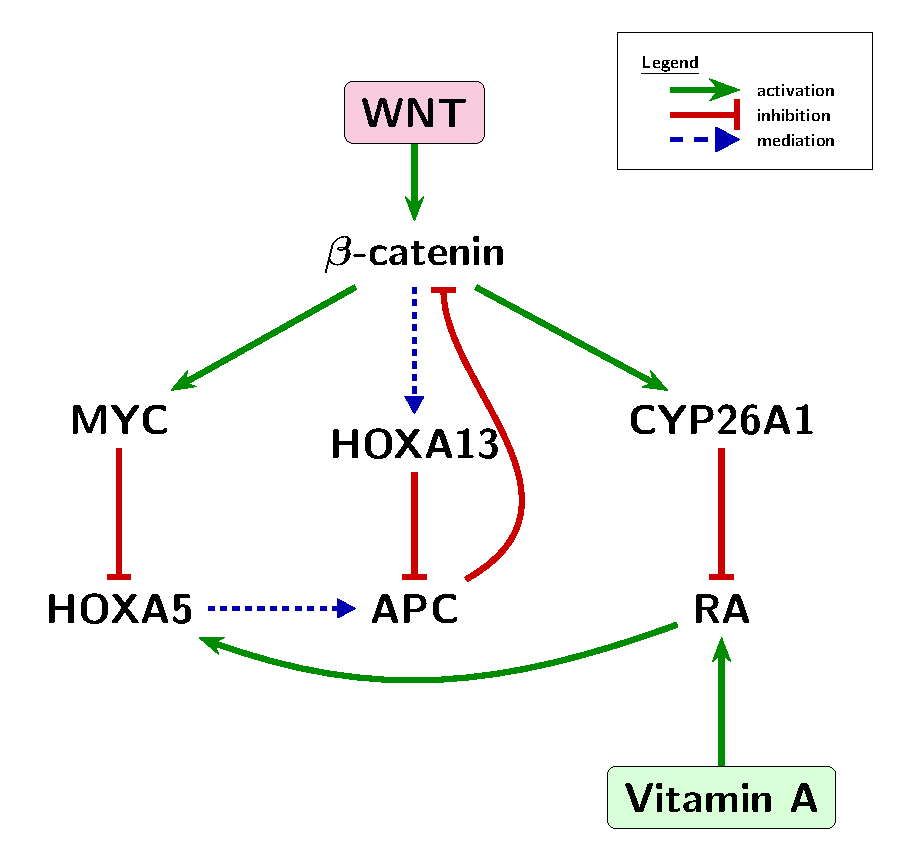
\includegraphics[width=\linewidth]{assets/model-original.pdf}
\end{minipage}\hfill
\begin{minipage}[c]{6.55in}
{\Display\bfseries\fontsize{29}{37}\selectfont Disease regimes\par}
\vspace{10pt}
{\fontsize{25}{33}\selectfont\renewcommand{\arraystretch}{1.1}
\setlength{\tabcolsep}{9pt}
\begin{tabular*}{\linewidth}{@{\extracolsep{\fill}}lrr@{}}
\toprule
Regime & $W$ & $\theta_P$\\
\midrule
Normal & 0.8 & 1.00\\
Early adenoma & 1.0 & 0.75\\
Advanced adenoma & 1.5 & 0.50\\
Severe APC loss & 2.0 & 0.25\\
\bottomrule
\end{tabular*}\par}
\Caption{$W$: WNT drive.\\$\theta_P$: APC functioning.}
\vspace{19pt}
{\Display\bfseries\fontsize{29}{37}\selectfont Seven states\par}
\Caption{$\mathbf z=(b,p,h_5,h_{13},m,r,c)$\\
$b$: $\beta$-catenin;\enspace $p$: APC\\
$h_5,h_{13}$: HOXA5, HOXA13\\
$m$: MYC;\enspace $r$: RA;\enspace $c$: CYP26A1}
\end{minipage}
\Caption{\textbf{Fig. 1.} Regulatory network.}

\Subhead{Nondimensional model}
Scale concentrations by characteristic values and time by $\beta$-catenin turnover, $d_B=1\,\mathrm{h}^{-1}$:
\Equation{1}{X=X_\ast x,\qquad \tau=d_Bt,\qquad
\varepsilon_X=\frac{d_B}{d_X}.}
Hill activation: $H_n(u;\kappa)=u^n/(\kappa^n+u^n)$. A dot below denotes $d/d\tau$.
\par\vspace{9pt}
\Equation{2}{
\begin{aligned}
\dot b &=
 W+\eta_{13}H_{n_H}(h_{13};\kappa_{13})
 -b-\lambda_Ppb-\lambda_5\frac{h_5b}{\kappa_5+b},
 \\[8pt]
\varepsilon_P\dot p &=
 \frac{1+\rho_5h_5}{1+\rho_Bb+\rho_{13}h_{13}}-D_P(\theta_P)p,
 \\[8pt]
\varepsilon_5\dot h_5 &=
 a_5+\eta_RH_1(r;\kappa_R)-h_5-\eta_M\frac{mh_5}{\kappa_M+m},
 \\[8pt]
\varepsilon_{13}\dot h_{13} &=
 a_{13}+\eta_{B13}H_{n_B}(b;\kappa_{B13})
 +\eta_{M13}H_{n_M}(m;\kappa_{M13})-h_{13},
 \\[8pt]
\varepsilon_M\dot m &=
 a_M+\eta_{BM}H_{n_B}(b;\kappa_{BM})-m,
 \\[8pt]
\varepsilon_R\dot r &= \mu_R(\tau)-r-\lambda_Ccr,
 \\[8pt]
\varepsilon_C\dot c &=
 a_C+\eta_{RC}H_1(r;\kappa_{RC})+\eta_{BC}H_{n_B}(b;\kappa_{BC})-c .
\end{aligned}}

\Subhead{APC functioning \& retinoid input}
\Equation{3}{\begin{aligned}
D_P(\theta_P)&=1+\delta_{P1}(1-\theta_P),\\[8pt]
\mu_R(\tau)&=\mu_0+A_R\!\left[1+\cos\!\left(\frac{2\pi\tau}{T_R}-\varphi\right)\right]\\[8pt]
&\quad+\frac{D_R}{2}
\left[\tanh q(\tau-\tau_1)-\tanh q(\tau-\tau_2)\right].
\end{aligned}}
\Caption{Radau reference; $\tau\in[0,150]$. ATRA pulse: $40\le\tau\le88$.}
\PanelEnd}

% ==================== 2. PINNs ====================
\sbox{\MiddleColumn}{\PanelStart{\MiddleWidth}
\SectionTitle{02}{PINNs \& identifiability}
\par\vspace{8pt}\noindent% Editable vector schematic of the forward PINN; neuron counts are abbreviated.
% Architecture checked against experiments/04-forward-pinn/forward-pinn-train-hybrid/model.py.
\begingroup
\begin{tikzpicture}[x=1in,y=1in,
  font=\fontsize{24}{29}\selectfont,
  connection/.style={line width=.85pt,draw=Garnet!26},
  flow/.style={-{Stealth[length=8pt,width=7pt]},line width=1.7pt,draw=Ink!70},
  neuron/.style={circle,minimum size=14pt,inner sep=0pt,
    draw=Garnet,line width=1.3pt,fill=Garnet!75},
  state/.style={circle,minimum size=14pt,inner sep=0pt,
    draw=DataBlue,line width=1.3pt,fill=DataBlue!18},
  loss/.style={rounded corners=8pt,minimum width=2.55in,
    minimum height=.80in,align=center,inner sep=5pt,line width=1.4pt}]
\path[use as bounding box] (0,0) rectangle (14.6,4.45);

% A prominent, fully connected neural network, with four hidden layers.
\filldraw[rounded corners=12pt,fill=Garnet!4,draw=Garnet!20,line width=1pt]
  (3.50,.94) rectangle (8.55,4.42);
\node[font=\bfseries\fontsize{30}{36}\selectfont,text=Garnet]
  at (6.025,4.05) {NEURAL NETWORK};
\node[font=\fontsize{24}{29}\selectfont] at (6.025,1.15)
  {4 hidden layers $\times$ 256\enspace\textbullet\enspace GELU};
\foreach \layer/\x in {1/4.05,2/5.35,3/6.65,4/7.95}{
  \foreach \j/\y in {1/3.47,2/3.03,3/2.59,4/1.70}
    \coordinate (h-\layer-\j) at (\x,\y);
}
\foreach \layer/\next in {1/2,2/3,3/4}
  \foreach \i in {1,...,4}
    \foreach \j in {1,...,4}
      \draw[connection] (h-\layer-\i) -- (h-\next-\j);

% Time is lifted to a fixed bank of 33 Fourier features.
\node at (.48,3.22) {Time};
\node[circle,draw=Ink!65,line width=1.6pt,minimum size=.48in,
  inner sep=0pt,font=\fontsize{30}{36}\selectfont] (time) at (.48,2.70) {$\tau$};
\filldraw[rounded corners=8pt,fill=PaleBlue,draw=DataBlue!45,line width=1.4pt]
  (1.24,1.70) rectangle (3.17,3.67);
\node[font=\bfseries\fontsize{25}{30}\selectfont] at (2.205,3.25) {Fourier};
\node[font=\fontsize{34}{40}\selectfont,text=DataBlue] at (2.205,2.70) {$\gamma(s)$};
\node at (2.205,2.08) {33 inputs};
\node at (2.205,1.18) {$s=\tau/T$};
\draw[flow] (time.east) -- (1.20,2.70);
\foreach \j in {1,...,4}
  \draw[connection,draw=DataBlue!45] (3.17,2.70) -- (h-1-\j);

% Seven outputs retain the model's canonical state order.
\node[font=\bfseries\fontsize{26}{32}\selectfont] at (9.94,4.05) {7 states};
\foreach \j/\y in {1/3.57,2/3.22,3/2.87,4/2.52,5/2.17,6/1.82,7/1.47}
  \coordinate (out-\j) at (9.50,\y);
\foreach \i in {1,...,4}
  \foreach \j in {1,...,7}
    \draw[connection,draw=DataBlue!38] (h-4-\i) -- (out-\j);
\draw[draw=Ink!45,line width=1.1pt] (10.95,1.34) -- (10.95,3.58);
\foreach \j/\label in {1/b,2/p,3/h_5,4/h_{13},5/m,6/r,7/c}{
  \draw[draw=Ink!35,line width=1.0pt] (out-\j) -- (10.95,0 |- out-\j);
  \node[state] at (out-\j) {};
  \node[anchor=west,fill=white,inner xsep=5pt,inner ysep=0pt]
    at ([xshift=.18in]out-\j) {$\label$};
}
\foreach \layer in {1,...,4}{
  \foreach \j in {1,...,4}
    \node[neuron] at (h-\layer-\j) {};
  \node[text=Garnet,font=\fontsize{26}{29}\selectfont]
    at (h-\layer-1 |- 0,2.16) {$\vdots$};
}

% Predictions feed all three forward losses; their sum trains the weights.
\node[loss,draw=DataBlue!60,fill=PaleBlue] (data) at (12.60,3.50)
  {\textbf{Data fit}\\$\mathcal L_{\rm data}$};
\node[loss,draw=Muted!55,fill=Paper] (initial) at (12.60,2.42)
  {\textbf{Initial state}\\$n\,\mathcal L_{\rm IC}$};
\node[loss,draw=Garnet!65,fill=Garnet!7] (physics) at (12.60,1.34)
  {\textbf{ODE residual}\\$\mathcal L_{\rm phys}$};
\foreach \name/\y in {data/3.50,initial/2.42,physics/1.34}{
  \draw[flow] (10.95,\y) -- (\name.west);
  \draw[draw=Garnet!65,line width=1.5pt] (\name.east) -- (14.23,\y);
}
\draw[draw=Garnet!65,line width=1.5pt] (14.23,3.50) -- (14.23,.47);
\node[circle,draw=Garnet,fill=white,inner sep=2pt,
  font=\fontsize{24}{29}\selectfont] (sum) at (14.23,.47) {$\Sigma$};
\draw[flow,draw=Garnet] (sum.west) -- (6.025,.47) -- (6.025,.91);
\node[fill=white,inner sep=4pt,font=\fontsize{24}{29}\selectfont,text=Garnet]
  at (10.00,.47) {Backpropagation\enspace\textbullet\enspace Adam $\to$ L-BFGS};
\node[font=\fontsize{25}{31}\selectfont] at (2.91,.47)
  {$\mathcal L_{\rm fwd}=\mathcal L_{\rm data}+\mathcal L_{\rm phys}+n\,\mathcal L_{\rm IC}$};
\end{tikzpicture}%
\endgroup
\par
\Equation{4}{\mathcal L_{\rm phys}=\frac{1}{N_c}\sum_k
\left\|\partial_\tau\widehat{\mathbf z}_k-
\mathbf F(\tau_k,\widehat{\mathbf z}_k;\boldsymbol\theta)\right\|^2.}
\Caption{Forward PINN,\textsuperscript{1} implying IC $n=20$.}
\par\vspace{10pt}\noindent% Generated by figures/forward_plot.py; ATRA annotations are native LaTeX.
\begingroup
\begin{tikzpicture}[x=1in,y=1in]
\node[anchor=south west,inner sep=0pt] at (0,0) {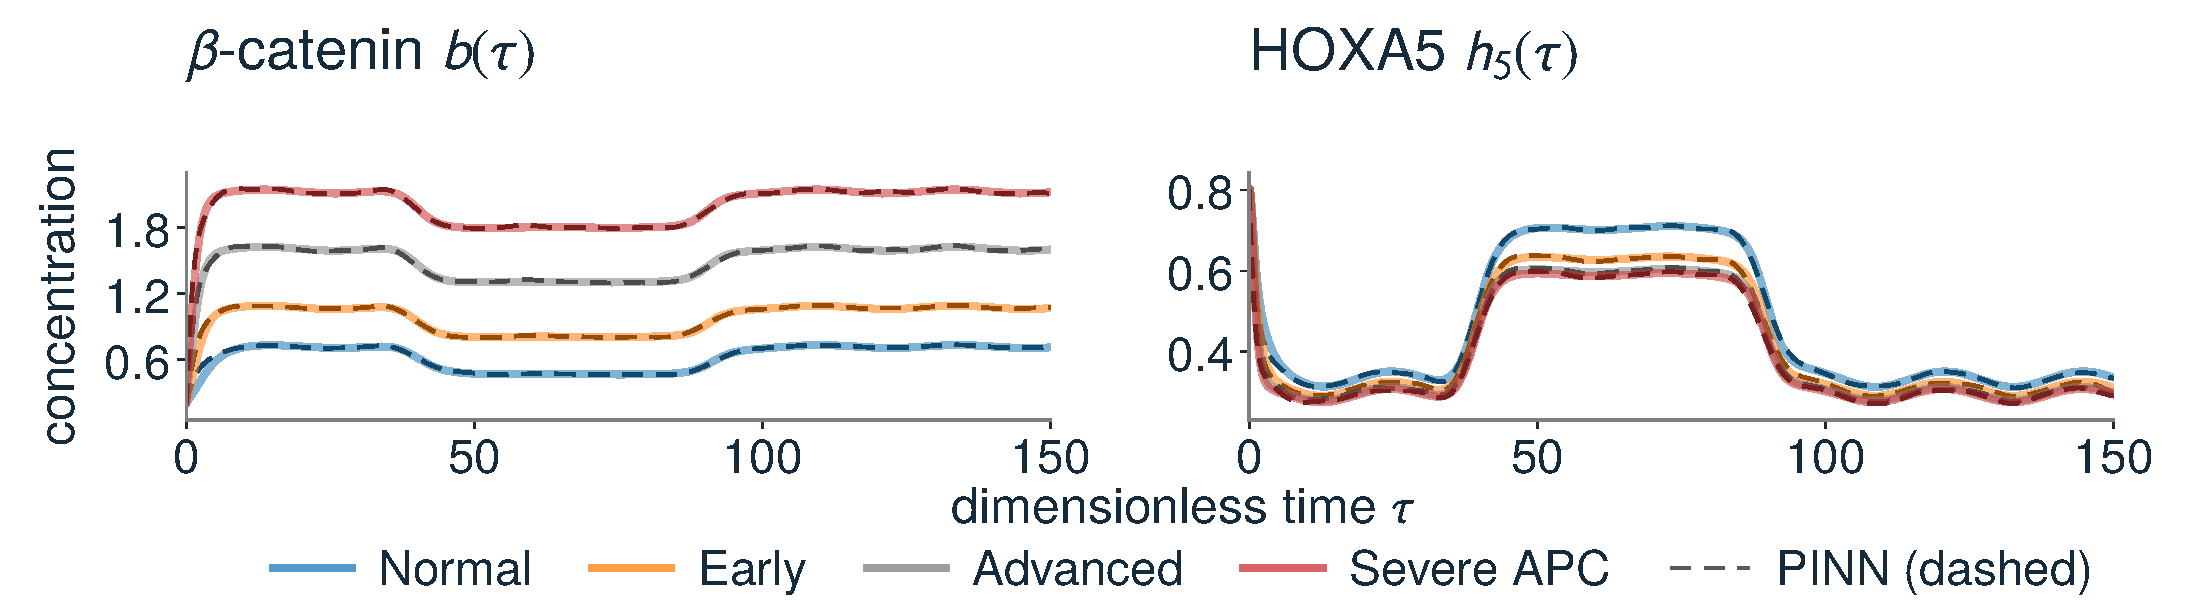
\includegraphics[width=14.6in]{assets/forward.pdf}};
\draw[{Stealth[length=8pt,width=7pt]}-{Stealth[length=8pt,width=7pt]},draw=Ink!80,line width=1.7pt] (2.77738,2.97000) -- node[above=5pt,font=\fontsize{24}{29}\selectfont,text=Ink] {ATRA} (4.62104,2.97000);
\draw[{Stealth[length=8pt,width=7pt]}-{Stealth[length=8pt,width=7pt]},draw=Ink!80,line width=1.7pt] (9.86395,2.97000) -- node[above=5pt,font=\fontsize{24}{29}\selectfont,text=Ink] {ATRA} (11.70761,2.97000);
\end{tikzpicture}%
\endgroup
\par
\Caption{\textbf{Fig. 2.} Forward PINN solution of the ODE system, four regimes.}

\Subhead{Inverse PINN: recovering 36 parameters}
\Equation{5}{\mathbf r_k=
\widehat{\mathbf z}_{k+1}-\widehat{\mathbf z}_k
-\tfrac{1}{2}\Delta\tau_k\big(\mathbf F_k+\mathbf F_{k+1}\big).}
\par\vspace{6pt}\noindent% Generated by figures/treatment_plot.py; the ATRA arrow is drawn in the PDF.
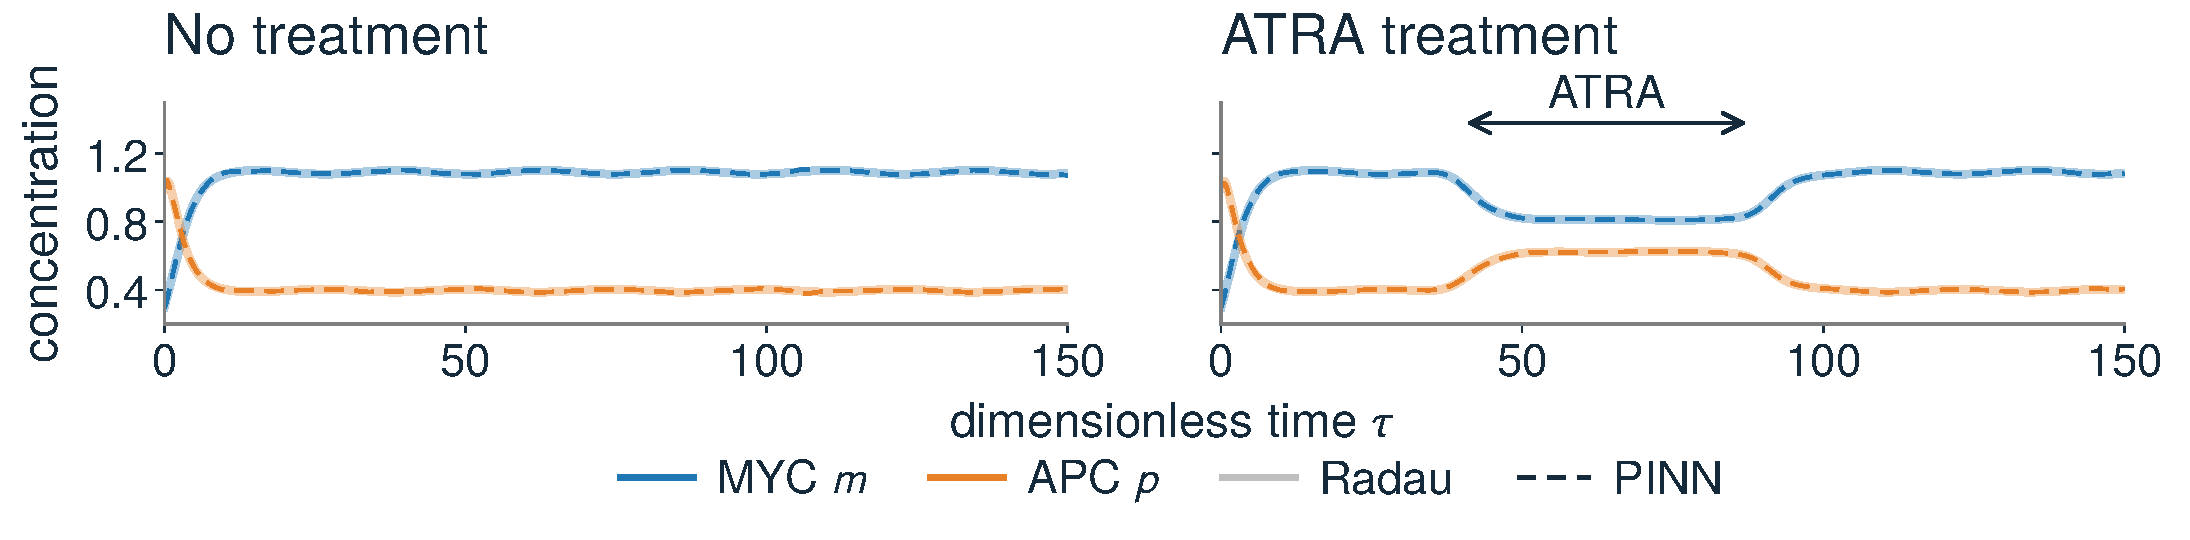
\includegraphics[width=14.6in]{assets/normal_pinn.pdf}
\par
\Caption{\textbf{Fig. 3.} Inverse PINN fit of Normal regime depending on treatment.}
\par\vspace{6pt}
{\TableFont\renewcommand{\arraystretch}{1.10}
\begin{tabular*}{\linewidth}{@{\extracolsep{\fill}}lrrrrr@{}}
\toprule
Method & Normal & Early & Advanced & Severe & Total\\
\midrule
\InverseCompactRows
\bottomrule
\end{tabular*}\par}
\Caption{\textbf{Table 1.} Parameters within 10\% error margin.}

\Subhead{Recovered vs. true parameters}
\par\vspace{7pt}
\begin{minipage}[c]{7.65in}
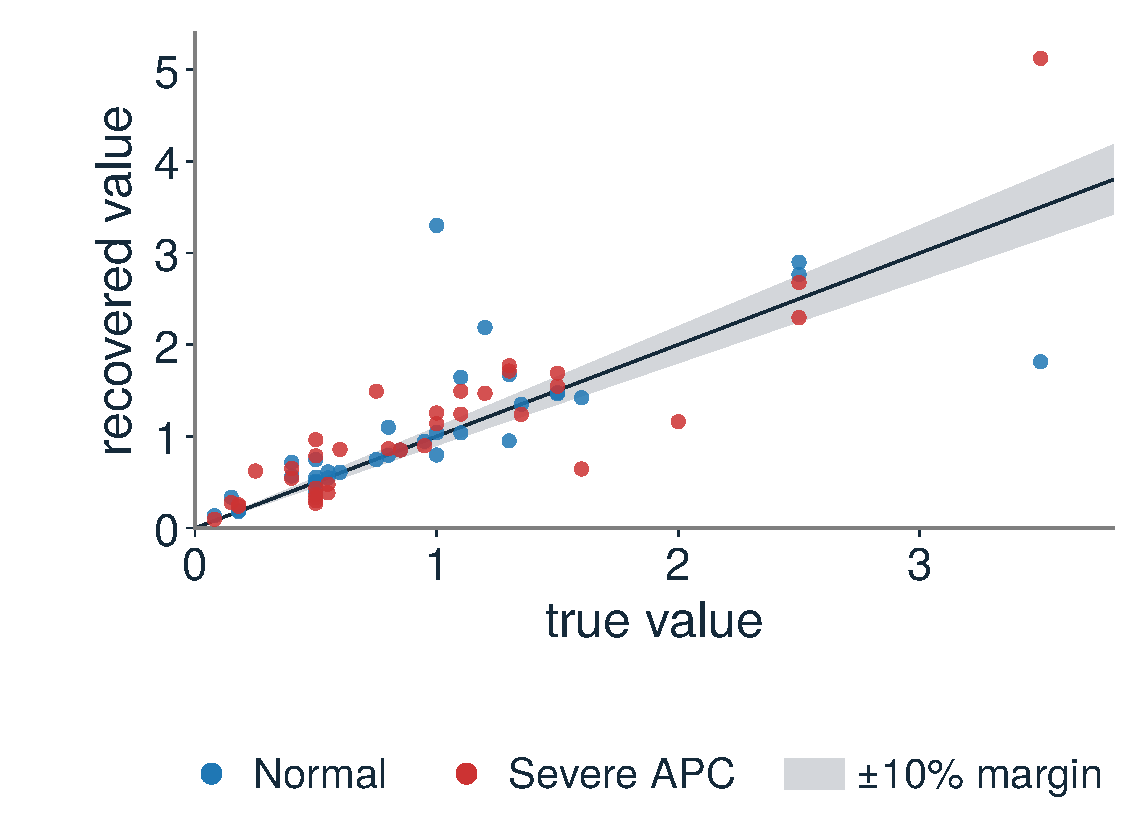
\includegraphics[width=\linewidth]{assets/parity.pdf}
\end{minipage}\hfill
\begin{minipage}[c]{6.50in}
{\Display\bfseries\fontsize{27}{35}\selectfont Local Fisher counts\par}
\vspace{10pt}
{\fontsize{24}{31}\selectfont\renewcommand{\arraystretch}{1.15}
\begin{tabular*}{\linewidth}{@{\extracolsep{\fill}}lrrr@{}}
\toprule
& I & W & N\\
\midrule
\FisherCompactRows
\bottomrule
\end{tabular*}\par}
\Caption{I: identifiable\\W: weak\\N: non-identifiable}
\end{minipage}
\Caption{\textbf{Fig. 4.} 36 parameters recovery results for inverse PINN.}
\PanelEnd}

% ==================== 3. NEURAL-MECHANISTIC HYBRID ====================
\sbox{\RightColumn}{\PanelStart{\RightWidth}
\SectionTitle{03}{Neural–mechanistic hybrid}
\Equation{6}{\begin{aligned}
\eta_{BM}H_{n_B}(b;\kappa_{BM})&\longrightarrow f_\phi(b),\qquad f_\phi(0)=0,\\[9pt]
\varepsilon_M\dot m&=\textcolor{Garnet}{a_M}+
\textcolor{DataBlue}{f_\phi(b)}-m.
\end{aligned}}
\Caption{$f_\phi$: shared $2\times5$ tanh network.\textsuperscript{2} Joint integral fit; L2 penalty $10^{-8}$.\\
Replace $(\eta_{BM},\kappa_{BM})$: 36 $\to$ 34 inverse parameters.}
\par\vspace{8pt}
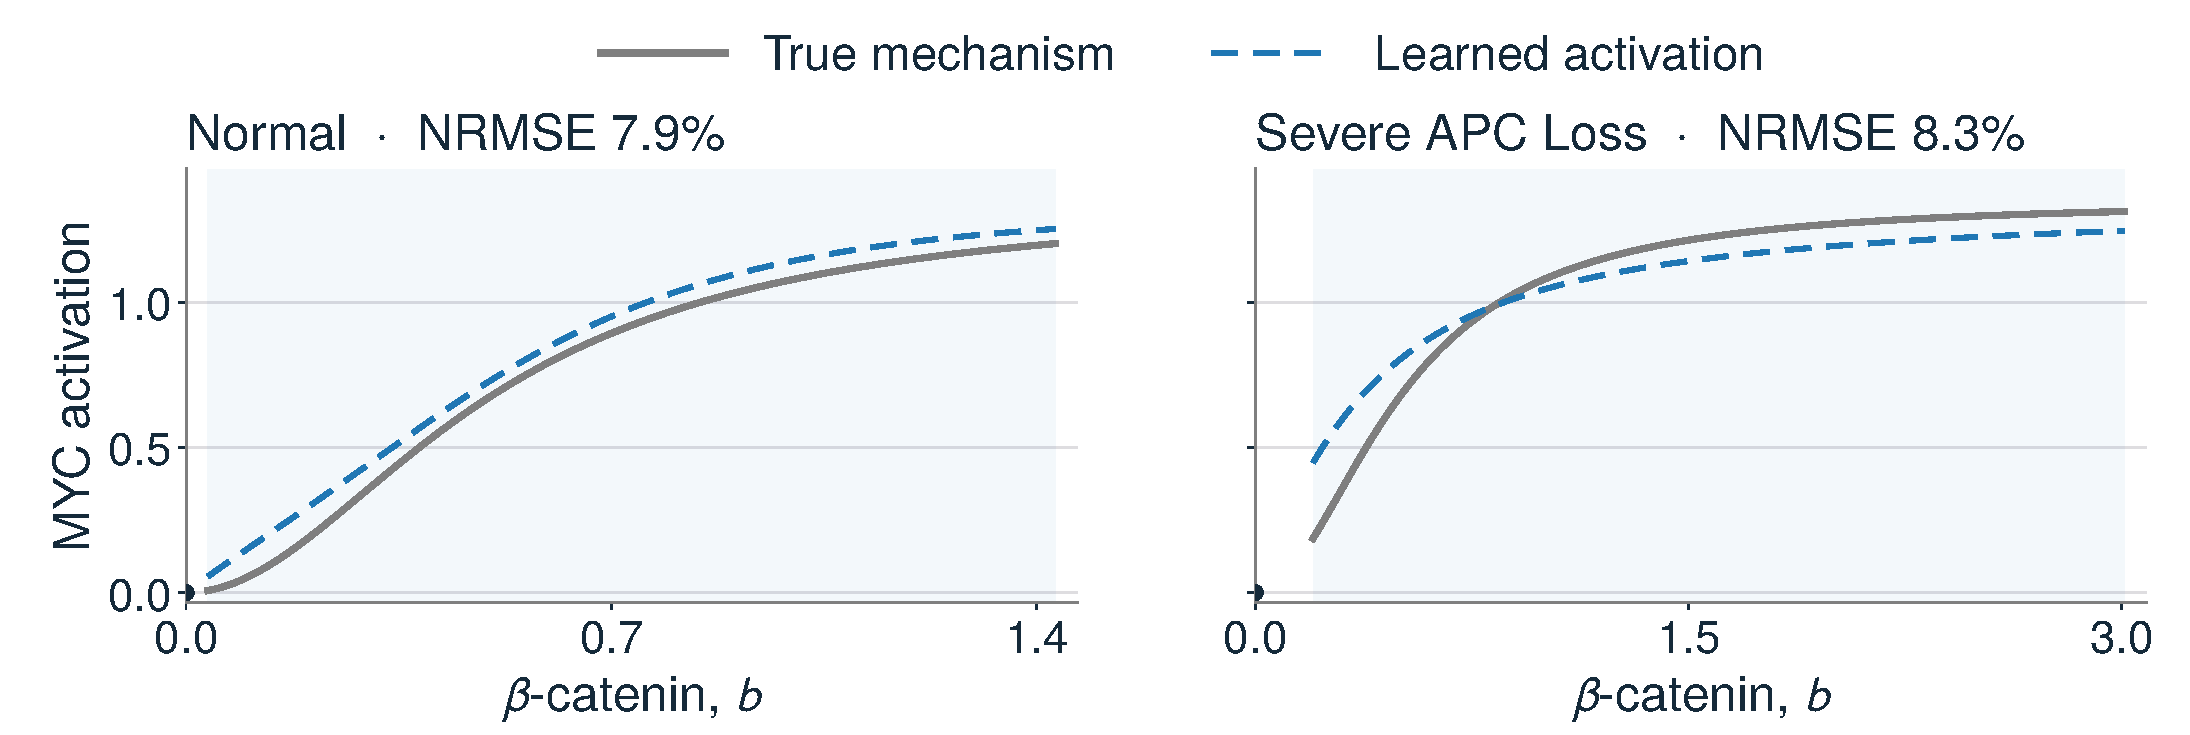
\includegraphics[width=\linewidth]{assets/learned-myc.pdf}
\Caption{\textbf{Fig. 5.} Learned MYC activation; dots mark $f_\phi(0)=0$.}

\Subhead{Parameter \& function recovery}
{\fontsize{25}{33}\selectfont\renewcommand{\arraystretch}{1.12}
\begin{tabular*}{\linewidth}{@{\extracolsep{\fill}}lrrr@{}}
\toprule
Learned term & Control & Hybrid & NRMSE (\%)\\
\midrule
\HybridRows
\bottomrule
\end{tabular*}\par}
\Caption{\textbf{Table 2.} Parameters within 10\% error margin, 4 regimes.}

\Subhead{Basal–neural compensation\textsuperscript{3}}
\Equation{7}{a_M+f_\phi(b)=(a_M+c)+\big[f_\phi(b)-c\big].}

\Subhead{Designed knockdowns}
{\fontsize{25}{33}\selectfont\renewcommand{\arraystretch}{1.10}
\begin{tabular*}{\linewidth}{@{\extracolsep{\fill}}llrr@{}}
\toprule
Basal & Knockdown & Normal & Severe\\
\midrule
\DoseRows
\midrule
\ProtocolRows
\bottomrule
\end{tabular*}\par}
\Caption{\textbf{Table 3.} Hybrid basal-parameter error (\%) under each knockdown.}

\Subhead{Mechanistic vs. hybrid errors}
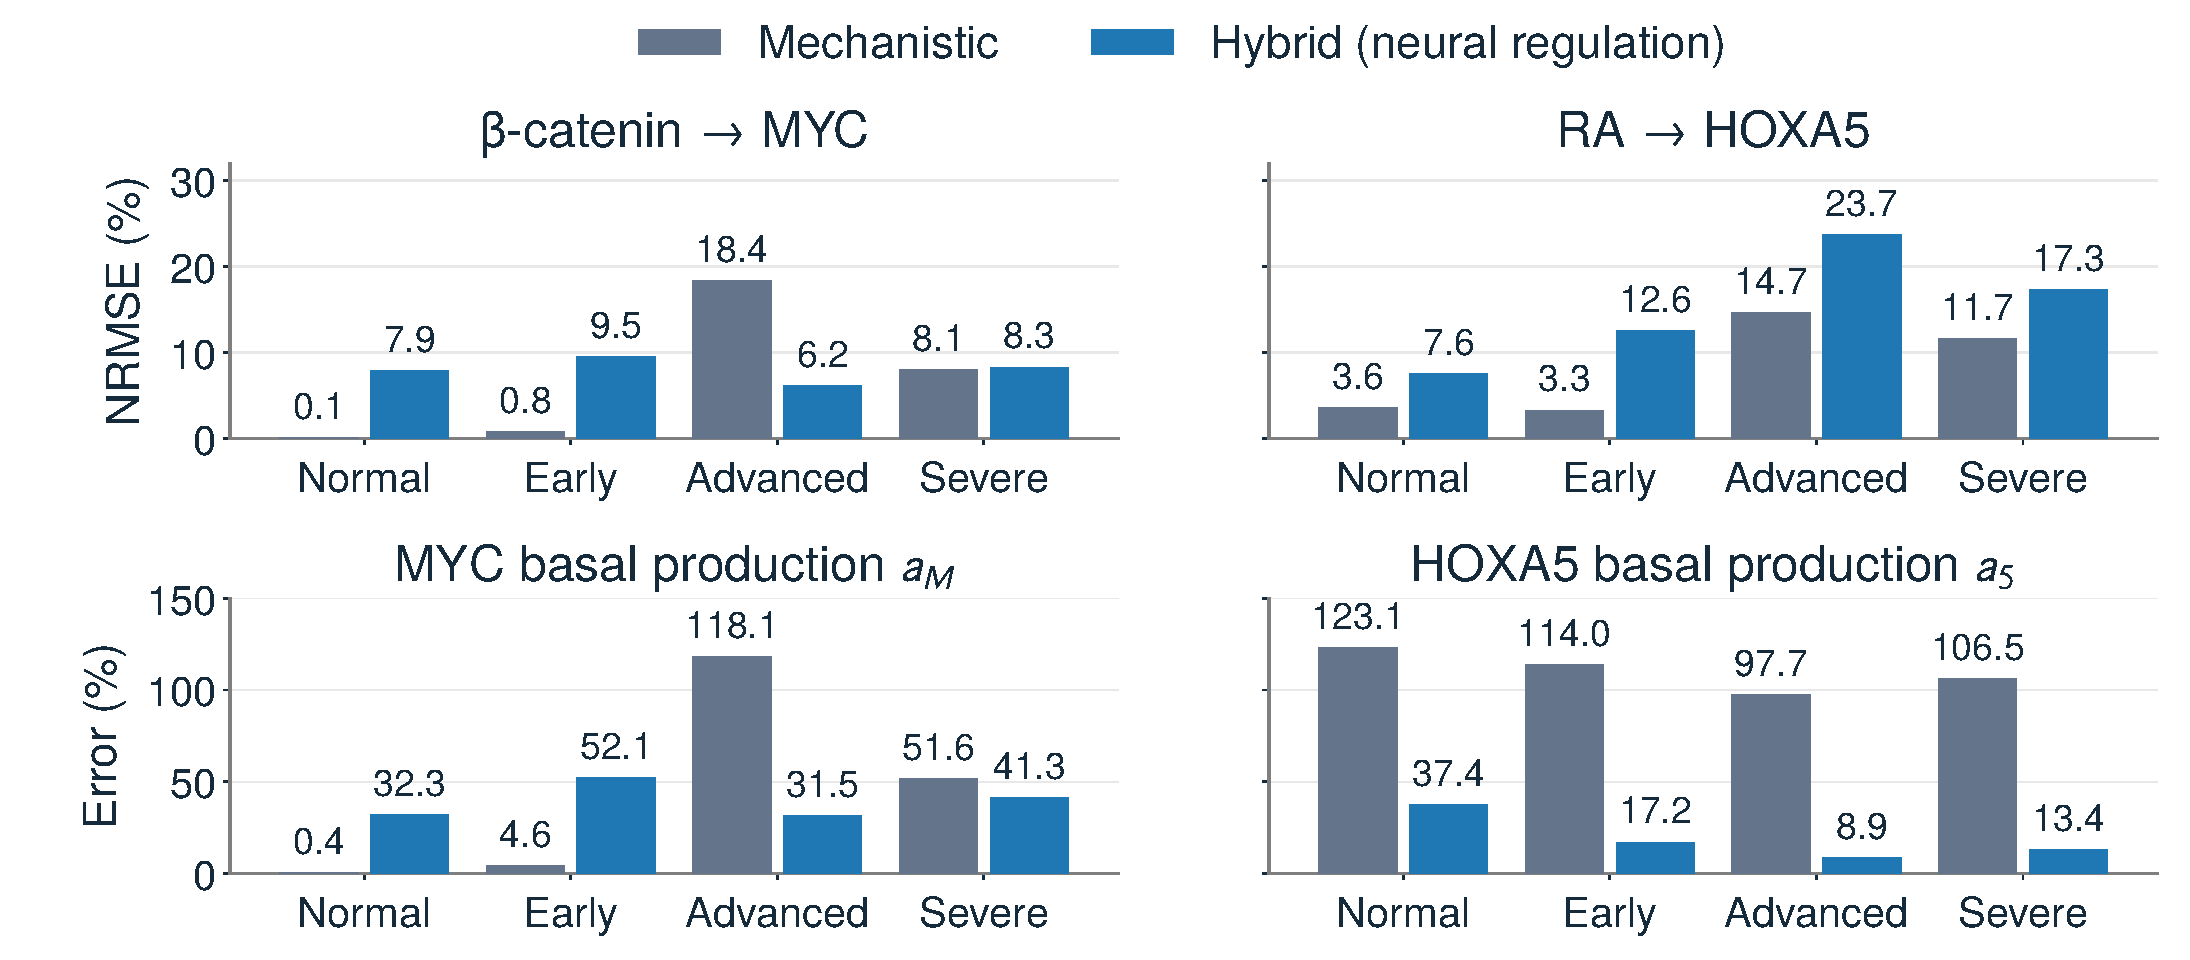
\includegraphics[width=\linewidth]{assets/hybrid-errors.pdf}
\Caption{\textbf{Fig. 6.} Mechanistic vs. hybrid errors, full inverse-PINN fits.}
\PanelEnd}

\sbox{\FooterBox}{\begin{minipage}{\LiveWidth}
{\color{Rule}\hrule height 1.5pt}\vspace{9pt}
{\fontsize{21}{26}\selectfont\setlength{\parindent}{0pt}\raggedright
\begin{minipage}[t]{.31\linewidth}\raggedright
{\bfseries References}\enspace
[1] Raissi et al. \textit{J. Comput. Phys.} 378 (2019).
\href{https://doi.org/10.1016/j.jcp.2018.10.045}{doi:10.1016/j.jcp.2018.10.045}.\par
\end{minipage}\hfill
\begin{minipage}[t]{.31\linewidth}\raggedright
[2] Rackauckas et al. Universal differential equations.
\href{https://arxiv.org/abs/2001.04385}{arXiv:2001.04385} (2020).\par
\end{minipage}\hfill
\begin{minipage}[t]{.34\linewidth}\raggedright
[3] Loman \& Baker. Functional and parametric identifiability for UDEs.
\href{https://arxiv.org/abs/2510.14140}{arXiv:2510.14140} (2025).\par
\end{minipage}\par}
\end{minipage}}
\typeout{MEASURE left=\the\dimexpr\ht\LeftColumn+\dp\LeftColumn\relax}
\typeout{MEASURE middle=\the\dimexpr\ht\MiddleColumn+\dp\MiddleColumn\relax}
\typeout{MEASURE right=\the\dimexpr\ht\RightColumn+\dp\RightColumn\relax}
\CheckHeight{title}{\TitleBox}{\LogoPanelHeight}
\CheckHeight{left}{\LeftColumn}{\BodyHeight}
\CheckHeight{middle}{\MiddleColumn}{\BodyHeight}
\CheckHeight{right}{\RightColumn}{\BodyHeight}
\CheckHeight{footer}{\FooterBox}{1.0in}

\begin{frame}[plain,t]
\begin{tikzpicture}[remember picture,overlay]
\fill[Garnet] (current page.north west) rectangle
  ([yshift=-4.20in]current page.north east);
\node[anchor=north west,inner sep=0pt,fill=white,rounded corners=16pt,
  minimum width=\LogoPanelWidth,minimum height=\LogoPanelHeight] (logopanel) at
  ([xshift=\Margin,yshift=-\TitleTop]current page.north west) {};
\node[inner sep=0pt] at (logopanel.center)
  {
\includegraphics[width=\LogoWidth]{assets/swarthmore-logo.pdf}};
\node[anchor=west,inner sep=0pt] at
  ([xshift=\dimexpr\Margin+\LogoPanelWidth+\TitleGap\relax,yshift=-\dimexpr\TitleTop+.5\LogoPanelHeight\relax]current page.north west) {\usebox{\TitleBox}};
\fill[white] ([xshift=.92in,yshift=-4.40in]current page.north west) rectangle
  ([xshift=\dimexpr\Margin+\LeftWidth+.18in\relax,yshift=-34.10in]current page.north west);
\fill[white] ([xshift=\dimexpr\Margin+\LeftWidth+\Gutter-.18in\relax,yshift=-4.40in]current page.north west) rectangle
  ([xshift=\dimexpr\Margin+\LeftWidth+\Gutter+\MiddleWidth+.18in\relax,yshift=-34.10in]current page.north west);
\fill[white] ([xshift=\dimexpr\Margin+\LeftWidth+\Gutter+\MiddleWidth+\Gutter-.18in\relax,yshift=-4.40in]current page.north west) rectangle
  ([xshift=-.92in,yshift=-34.10in]current page.north east);
\node[anchor=north west,inner sep=0pt] at
  ([xshift=\Margin,yshift=-\BodyTop]current page.north west) {\usebox{\LeftColumn}};
\node[anchor=north west,inner sep=0pt] at
  ([xshift=\dimexpr\Margin+\LeftWidth+\Gutter\relax,yshift=-\BodyTop]current page.north west) {\usebox{\MiddleColumn}};
\node[anchor=north west,inner sep=0pt] at
  ([xshift=\dimexpr\Margin+\LeftWidth+\Gutter+\MiddleWidth+\Gutter\relax,yshift=-\BodyTop]current page.north west) {\usebox{\RightColumn}};
\node[anchor=north west,inner sep=0pt] at
  ([xshift=\Margin,yshift=-\FooterTop]current page.north west) {\usebox{\FooterBox}};
\end{tikzpicture}
\end{frame}
\end{document}
